

\documentclass[../../e3_tp2_main.tex]{subfiles}

\begin{document}
\chapter{}

Se denomina \textit{hazard} a los \textit{glitches} causados por la estructura del circuitos y los delays de propagaci\'on de las compuertas. Estos ocurren cuando la salida toma moment\'aneamente un valor que no se corresponde con lo establecido por la tabla de verdad del circuito. Existen dos tipos de \textit{hazards}: din\'amicos y est\'aticos.
\begin{itemize}
	\item Din\'amico: cuando la salida cambia, oscila entre 0 y 1 moment\'aneamente antes de establecerse. Sucede cuando existen multiples caminos para que una se\~nal se propague. 
	\item Est\'atico: la salida cambia cuando deber\'ia mantenerse. Al usar el m\'etodo de mapas de Karnaugh con suma de productos para obtener la funci\'on l\'ogica de m\'inimo costo de una tabla de verdad, usualmente quedan 1 adyacentes que no comparten grupo. Las transiciones entre estos estados tienen un riesgo de \textit{hazards} est\'aticos. 
\end{itemize}
Se pueden observar ejemplos de ambos tipos en la figura \ref{fig:ej_3_hazards}.


\begin{figure}[H]	%ejemplo hazards
	\centering
	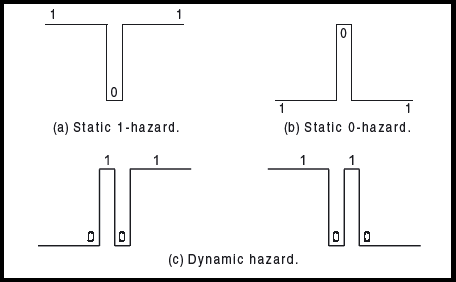
\includegraphics[width=0.35\textwidth]{hazard.png}
	\caption{\textit{Glitches} est\'aticos y din\'amicos \protect\footnotemark}
	\label{fig:ej_3_hazards}
\end{figure}

\footnotetext{Imagen extra\'ida de: \url{http://www.electronicsengineering.nbcafe.in/hazards-in-digital-circuit/} (13/10/18)}


Para evitar los \textit{hazards} est\'aticos, se usan funciones l\'ogicas resultantes de agregar grupos extras al mapa de Karnaugh de manera tal que todos los 1 adyacentes compartan grupo. Estos grupos extra son redundantes, por lo que van a aumentar el costo de la funci\'on.

\begin{figure}[H]	%kmap
	\centering
	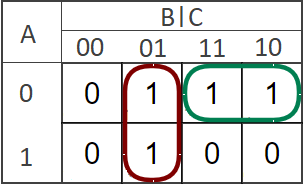
\includegraphics[width=0.15\textwidth]{kmap.png}
	\caption{Mapa de Karnaugh utilizado. Resoluci\'on de menor costo por suma de productos. Si se quisiera reducir el riesgo de \textit{hazards}, se deber\'ia agregar otro grupo que contenga a 001 y 011.}
	\label{fig:ej_3_kmap}
\end{figure}

Del mapa de Karnaugh de la figura \ref{fig:ej_3_kmap} se obtiene la funci\'on l\'ogica de menor costo de la salida:
$$Y = A'\cdot B+B'\cdot C$$
Se implement\'o esta funci\'on y se pudieron observar \textit{hazards}, como muestras las figuras \ref{fig:ej_3_up_haz} y \ref{fig:ej_3_down_haz} \protect\footnotemark. 

\begin{figure}[H]	%000->001 up hazard
	\centering
	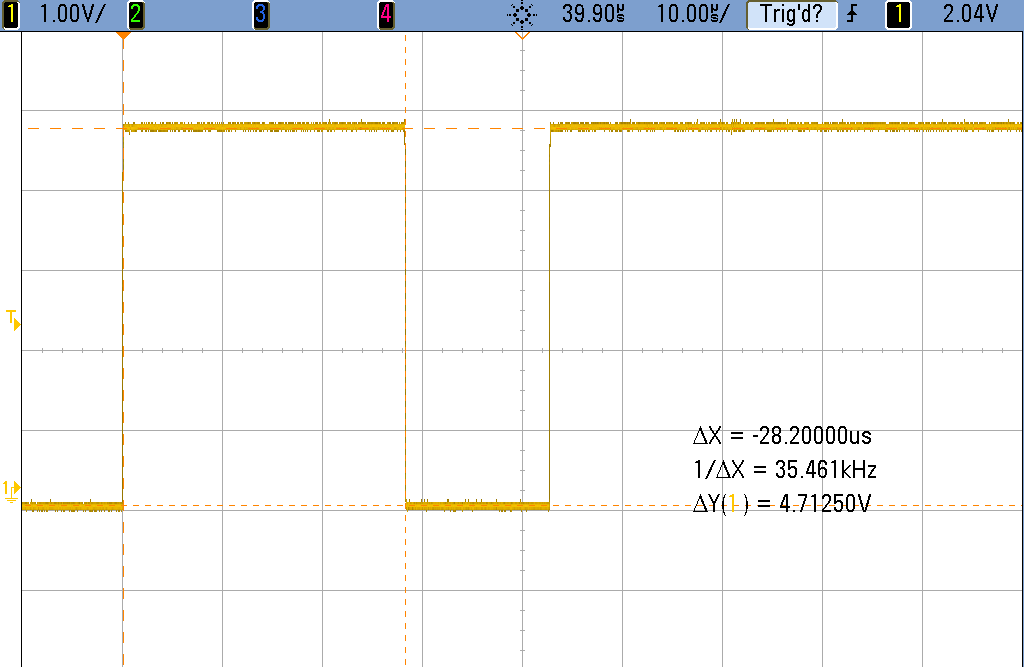
\includegraphics[width=0.33\textwidth]{000-001_haz.png}
	\caption{\textit{Hazard} din\'amico medido en la transici\'on 000\,$\rightarrow$\,001, donde la salida cambia de 0 a 1.}
	\label{fig:ej_3_up_haz}
\end{figure}


\begin{figure}[H]	%011->111 down hazard
	\centering
	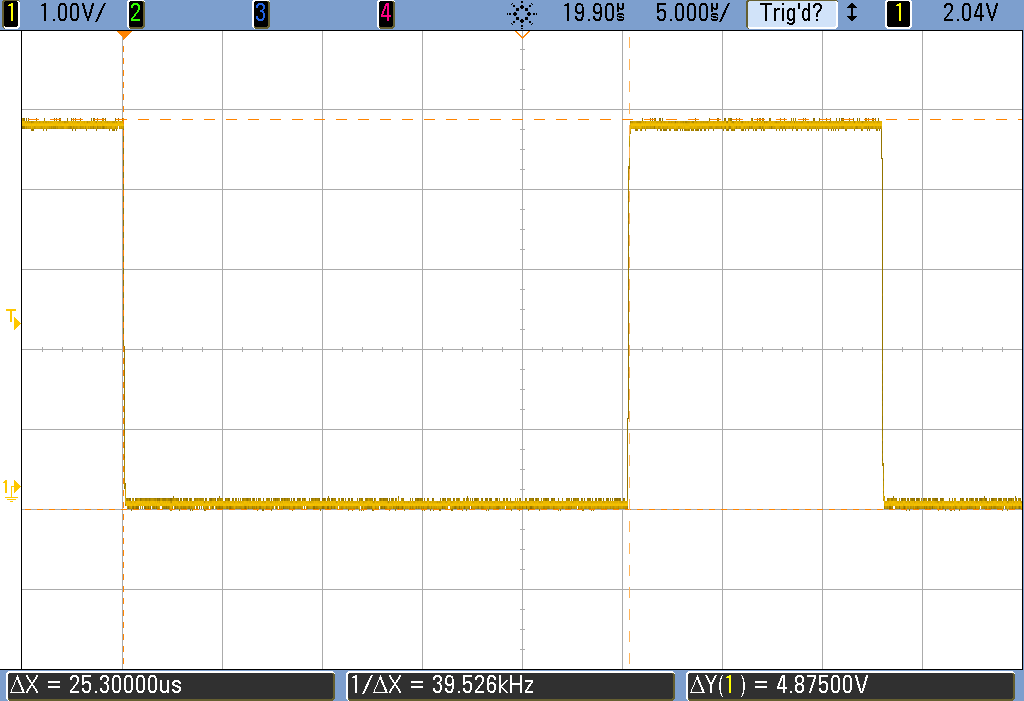
\includegraphics[width=0.33\textwidth]{011-111_haz.png}
	\caption{\textit{Hazard} din\'amico medido en la transici\'on 011\,$\rightarrow$\,111, donde la salida cambia de 1 a 0.}
	\label{fig:ej_3_down_haz}
\end{figure}



\footnotetext{Los \textit{hazards} no se observaron todas las veces que se realizaron estas transiciones, sino espor\'adicamente.}

\end{document}